\section{User Guide}
\subsection{Compile and install }
\subsubsection{Requirements }
This software has currently support only for GNU/Linux systems, as the cursor control is platform-dependent, but as it has a modular design it can be easily extended for being used on Windows or Mac platforms. Nevertheless we do not have any early plans of porting it to other platforms. 

The requirements for compiling and using the software are:
\begin{itemize}
\item CMAKE (minimum version 2.8)
\item OpenCV (v2.4.6.1).
\item X11 (GNU/Linux libraries that allow the interface with the X server for controlling the cursor). 
\end{itemize}


\subsubsection{Compiling}
\paragraph{Using CMake }
The folder structure used is the typical of a CMake project. In order to compile using the terminal follow this steps: 
\begin{enumerate}
 \item Open a terminal in the build directory (gecko/build). 
 \item Enter the command ``cmake ..''
 \item Enter the command ``make''
\end{enumerate}

\paragraph{Using QtCreator}
To open the software as a QtCreator project, the only thing needed is to open the main CMakeLists.txt (gecko/CMakeLists.txt) with QtCreator. This will parse the whole project. 
Afterwards, press the ``build'' icon to build the project. 


\subsection{Running the software}

In order to execute the software, press the convinient button of the QtCreator IDE or open a terminal in the bin directory (gecko/bin) and enter the command ``./gecko''. 

Once the code is compiled and started, a first window will appear with the information about the software. After pressing enter to continue, this menu will pop up: 
\begin{center}
\fbox{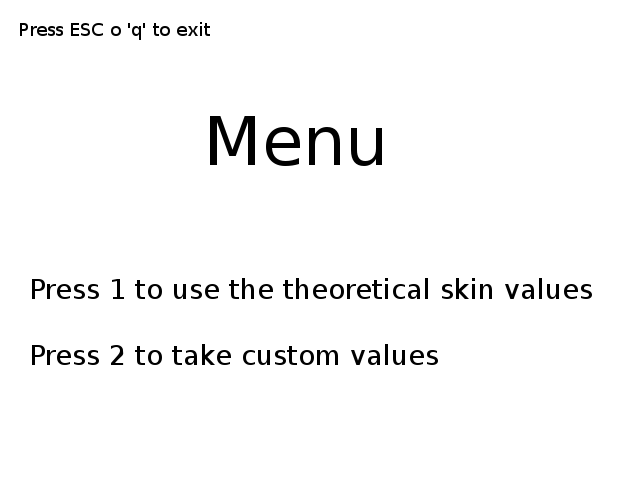
\includegraphics[scale=0.5]{../../img/menu.png} }
\end{center}

\vspace{1cm}
The first option will take the theoretical HSV skin values proposed in [1]. Afterwards, the application will allow us to adjust those HSV ranges to adecuate them to the room's conditions. 
Once all the adjustments are done, pressing ENTER will start the program. 

The second option will pop up a window with a green square in the middle. Place the hand so that the square is in the middle of your palm and press ENTER. The program will automatically calculate the HSV range of your skin. Afterwards you will be able once more to manually adjust those ranges. Pressing ENTER one last time will start the program. 
\\
 
The main program will track the hand and trace two circles, the first one around the palm and the second one surrounding the whole hand. The center of the palm is also shown, as well as the angle described by the hand. 

There are different functionalities implemented in this software. 
\begin{itemize}
\item Open hand: the mouse moves with the hand's movement.
\item Closed hand: click.
\item ``Victory sign'': the gedit text editor is opened.
\item ``Gun or L sign'': a terminal is opened. 
\end{itemize}

The two last functionalities may be changed using a configuration file named apps.config (gecko/data/apps.config). 

That configuration file contains the following lines:
\\[0.5cm]
\begin{center}
\$gedit\$ 3 \\
\$gnome-terminal\$ 4
\\[0.5cm]
\end{center}

The number 3 refers to the victory sign, and  4 to the gun or L sign. To change the functionality the only thing needed is to change the programs written between the two dollar signs with the wanted one. 

\begin{center}
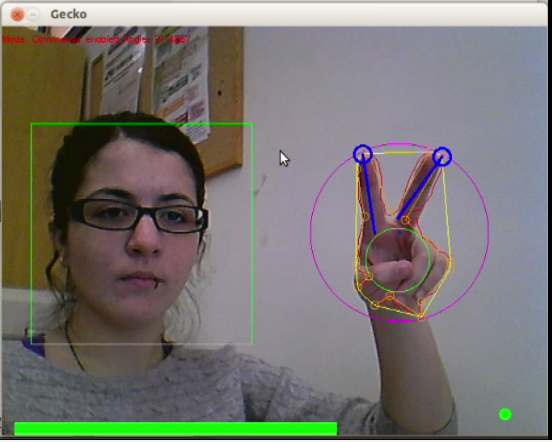
\includegraphics[scale=0.5]{images/victory.png} 
\end{center}

The user should take into account that when the program recognizes a gesture, a bar will appear in the window. In order to filter possible false positives, the user must remain in the same posture until the bar is completely filled for the correct execution of the task associated with the gesture, as it can be seen in the picture above. 


\newpage
